\documentclass[a4paper, 11pt]{article}
\usepackage{comment} % enables the use of multi-line comments (\ifx \fi) 
\usepackage{lipsum} %This package just generates Lorem Ipsum filler text. 
\usepackage{fullpage} % changes the margin
\usepackage{outline}
\usepackage{pmgraph}
\usepackage[utf8x]{inputenc}
\usepackage[T1]{fontenc}
\usepackage{esvect}
\usepackage{amsmath}
\usepackage{bm}
\usepackage{mathtools}
\usepackage{tcolorbox}
\usepackage{longtable}
\usepackage{physics}
\usepackage{gensymb}
%\usepackage[document]{ragged2e}
\usepackage{color}
\usepackage{multicol}
\usepackage{bm}
\usepackage{graphicx}
\usepackage{setspace}
\usepackage{amssymb}
\usepackage{amsmath}
\usepackage[nottoc]{tocbibind}
\usepackage[normalem]{ulem}
\usepackage{caption}
\usepackage{subcaption}
\usepackage{geometry}
\usepackage{layout}
\setlength{\voffset}{-1in}
\setlength{\hoffset}{-0.9in}
\setlength{\textwidth}{550pt}
\setlength{\textheight}{750pt}
\begin{document}
%Header-Make sure you update this information!!!!
\noindent
\large\textbf{Assignment Report} \hfill \textbf{Ramy Tanios} \\
\normalsize MECH764 \hfill 201404444 \\
Prof. Fadl Moukalled \hfill \\ \hfill Due Date: 24/4/2018

\section*{Introduction}
In this report, I will be presenting the results of the finite volume discretization method applied to the two dimensional transient heat conduction equation
\begin{equation*} 
\frac{\partial\phi}{\partial t}-\kappa\nabla^2\phi=0,
\end{equation*}
 where $\kappa$ is the thermal diffusivity of the plate and $\phi$ is temperature. The transient term will be discretized using the \textbf{Backward Euler} scheme and the \textbf{Crank-Nicolson} scheme.
%----------------
\section*{Problem Statement}
In this problem, the thermal diffusivity $\kappa$ is constant such that $\kappa=1 \ \text{m.s}^{-1}.$ The computational domain studied is a square plate with length $L=1\text{m}$ and height $H=1 \text{m}$. The boundary conditions are such that the north boundary is insulated, i.e $\forall x \in [0,1],\forall t>0, \nabla\phi(x,H,t)=0$ (von Neumann BC) and the other boundaries are held at a constant temperature of 0$^{\circ}$C (Dirichlet BC), for $t>0$. At $t=0$, the plate has a uniform temperature distribution of 100$^{\circ}$C.
%----------------
\section*{Analytical Solution}
The analytical solution to this problem with the specified boundary conditions is: 
\begin{equation*}
\phi(x,y,t) = \sum_{m=1}^{\infty}\sum_{n=1}^{\infty} \frac{1600}{(2n-1)(2m-1)\pi^2} \sin(\frac{(2n-1)\pi x}{L})\sin(\frac{(2m-1)\pi y}{2H}) \mathrm{e}^{-\kappa\pi^2t(\frac{(2m-1)^2}{4H^2}+\frac{(2n-1)^2}{L^2})}
\end{equation*}
%----------------
\section*{Numerical Implementation}
The method is implemented using fortran90. The main program \textit{main.f90} calls the following subroutines: \textit{allocateArrays.f90, getAnalyticalSolution.f90, transfiniteInterpolation.f90, geometricQuantities.f90, surfaceVectors.f90, getFields.f90, getDiffusiveCoeff.f90, getConvectiveCoeff.f90} and the solver \textit{iterativeSolver.f90} . \\
Most importantly, the subroutine \textit{getAnalyticalSolution} generate the analytical solution on the 2D grid. Since the solution is of the form of an infinite sum, the series is truncated when the absolute difference between two consecutive terms is less than a specified tolerance, mainly $10^{-8}$. Also, the subroutine \textit{getDiffusiveCoeff.f90} adds the contribution of the diffusion term to the coefficients $a_E, a_W, a_S, a_N, a_C$ and $b_C$. In addition, the subroutine \textit{modifyCoefficientsForTransientSolving.f90} adds the transient term contribution to the source term $b_C$ and the coefficients $a_C$ .Finally, \textit{iterativeSolver.f90} solves for the variable $\phi$ using the \textbf{TDMA} method, applied to lines of constant indexing $i$ and $j$ in order to get a tridiagonal matrix for the system of equations $\textbf{A}\phi=\textbf{b}$. \\ 
Also, using the command \textit{call system("python plot2D.py")}, the main program will call a python script that uses the \textit{matplotlib} library for plotting the results.\\
In the module \textit{fields.mod}, the user can change the velocity field function, the diffusivity field distribution and may add a source term to the equation to be solved. Finally, the boundary conditions of the problem are initialized in the module \textit{boundaryConditions.mod} . In that module, the user can change and set the desired boundary conditions. Note that all the variables in that module are declared as one dimensional arrays of size $4$, where the first element corresponds the boundary condition at the north boundary, the second for the east boundary, the third for the south boundary and finally the fourth element for the east boundary of the domain.
%----------------
\section*{Analytical And Finite Volume Solution Results}
In the following section, I will present a comparision between the backward Euler and the Crank-Nicolson methods for the discretization of the transient term, as well as 2D plots for the variation of the temperature distribution $\phi$ across the plate for different times.The time step is set to $\Delta t=0.001 \ \text{sec}.$
The following plot represents a comparision between backward Euler and Crank-Nicolson scheme. The value plotted is the percentage difference between the analytical solution $\phi_{Exact}$ and the finite volume solution $\phi_{FVM}$, i.e 
\begin{equation*} 
P.E =  100|\frac{\phi_{Exact}-\phi_{FVM}}{\phi_{Exact}}|.
\end{equation*}
\begin{figure}[ht!]
  \centering
  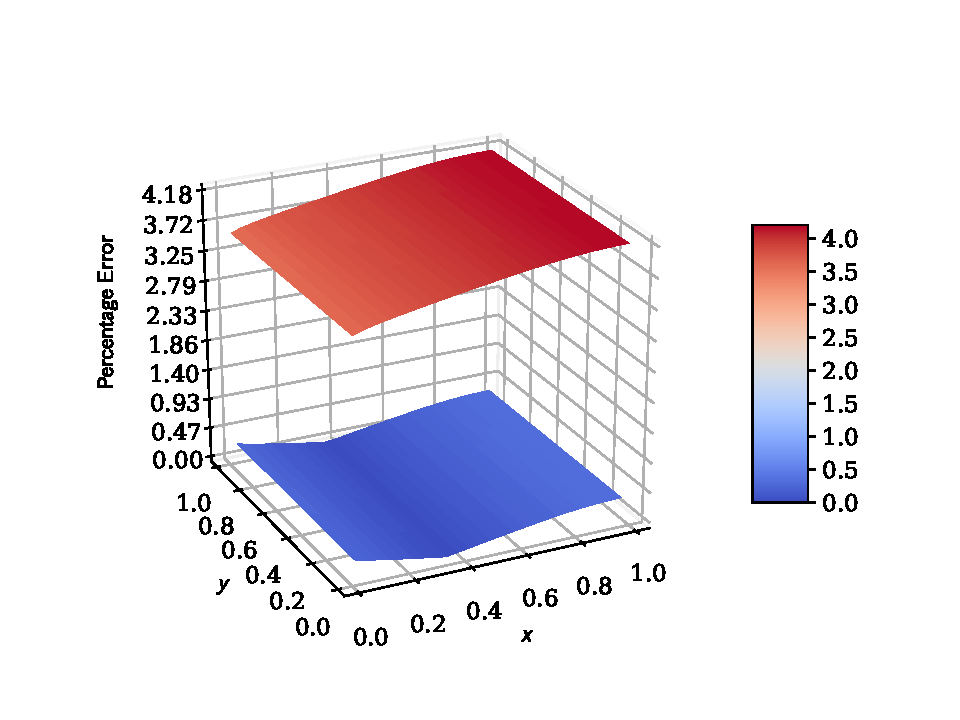
\includegraphics[width=1\linewidth]{0d5sec.pdf}
  \caption{The percentage error generated on the computational domain for the backward Euler method(upper surface) and the Crank-Nicolson method(lower surface) .}
  \label{fig:sub31}
\label{fig:sub32}
\end{figure}
It is clear that the Crank-Nicolson method which is second order provides a more accurate solution to the problem in comparison to the backward Euler which is first order. Finally, the following are plots of the $\phi$ distribution for different timings.
\begin{figure}[ht!]
\centering
\begin{subfigure}{0.5\textwidth}
  \centering
  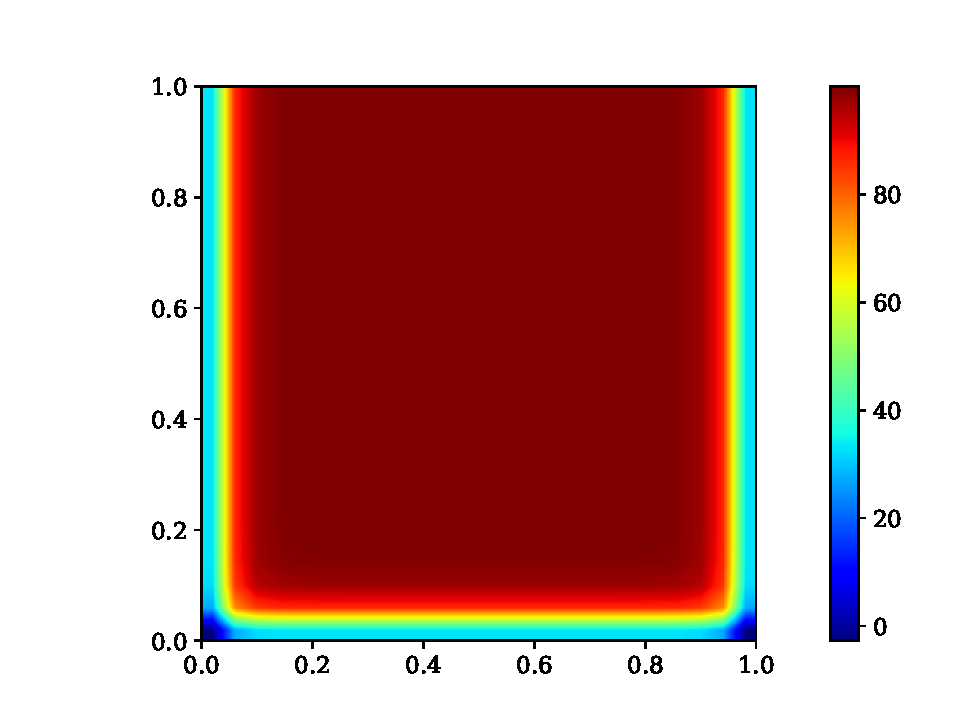
\includegraphics[width=1\linewidth]{0d00001sec.pdf}
  \caption{$t = 0.00001 \ \text{sec}$.}
  \label{fig:sub31}
\end{subfigure}%
\begin{subfigure}{0.5\textwidth}
  \centering
  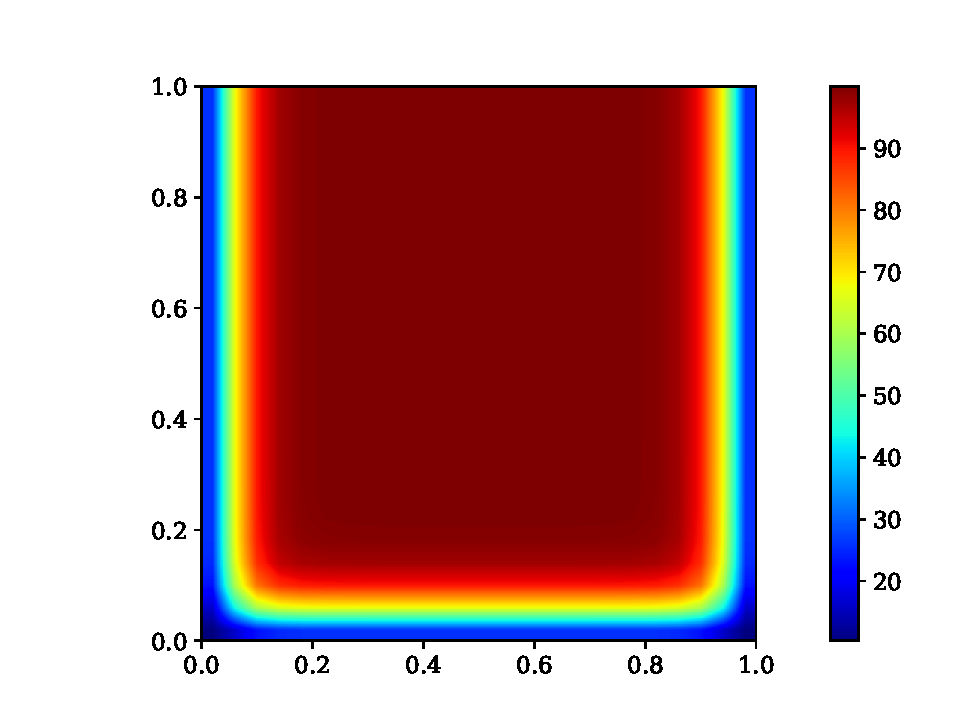
\includegraphics[width=1\linewidth]{0d001sec.pdf}
  \caption{$t = 0.001 \ \text{sec}$.}
  \label{fig:sub2}
\end{subfigure}
\caption{The temperature distribution over the plate for $t = 0.00001 \ \text{sec}$ and $t = 0.001 \ \text{sec}$.}
\label{fig:sub32}
\end{figure}
% 
\begin{figure}[ht!]
\centering
\begin{subfigure}{0.5\textwidth}
  \centering
  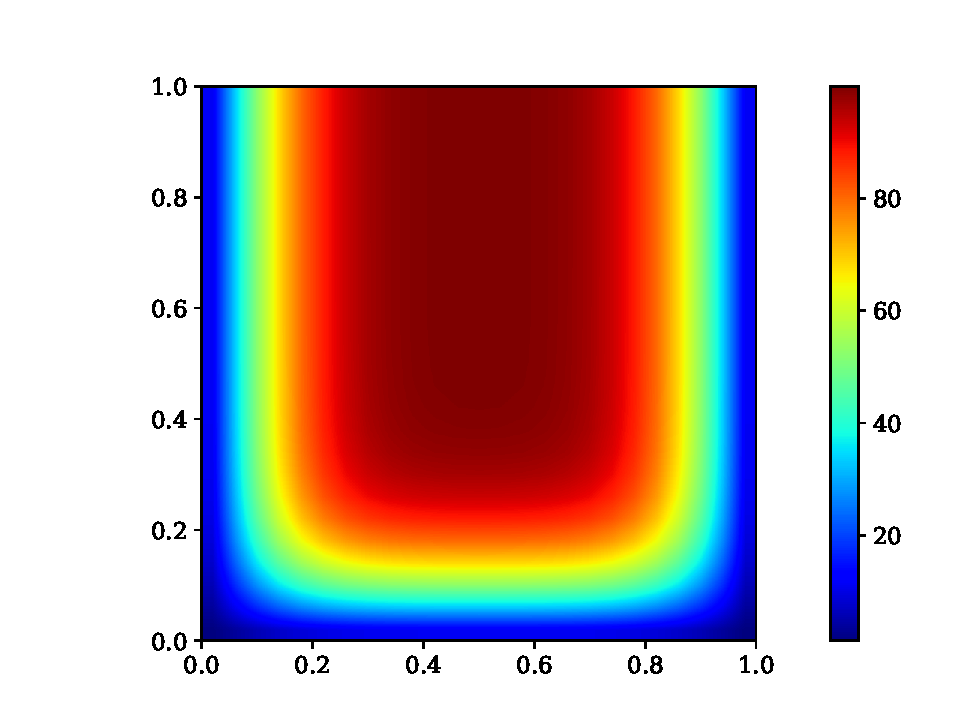
\includegraphics[width=1\linewidth]{0d01sec.pdf}
  \caption{$t = 0.01 \ \text{sec}$.}
  \label{fig:sub31}
\end{subfigure}%
\begin{subfigure}{0.5\textwidth}
  \centering
  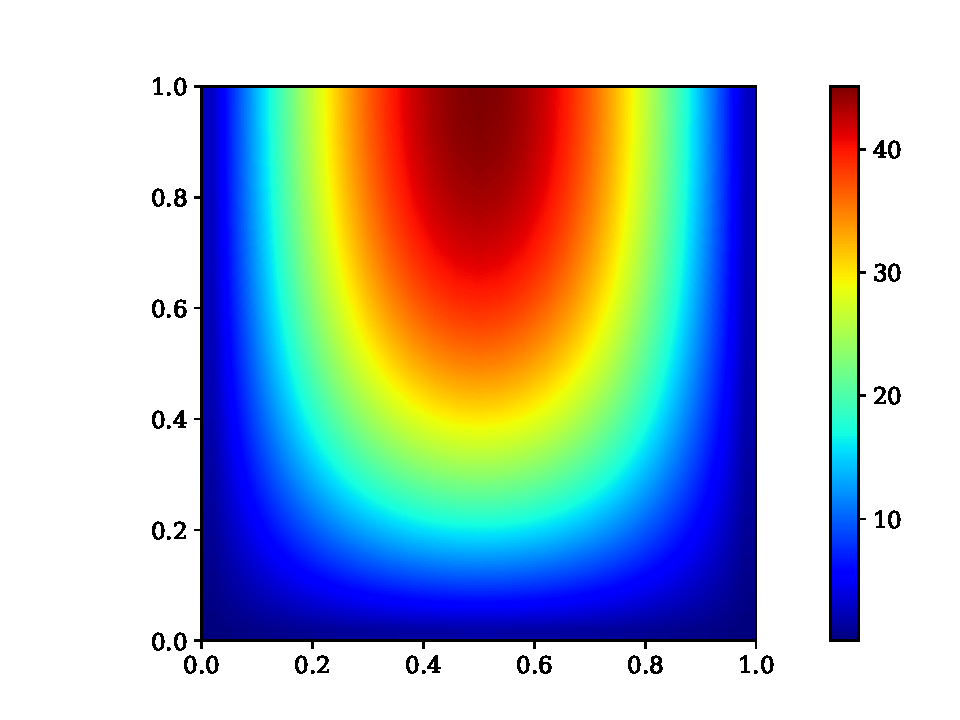
\includegraphics[width=1\linewidth]{0d1sec.pdf}
  \caption{$t = 0.1 \ \text{sec}$.}
  \label{fig:sub2}
\end{subfigure}
\caption{The temperature distribution over the plate for $t = 0.01 \ \text{sec}$ and $t = 0.1 \ \text{sec}$.}
\label{fig:sub32}
\end{figure}
\begin{figure}[ht!]
  \centering
  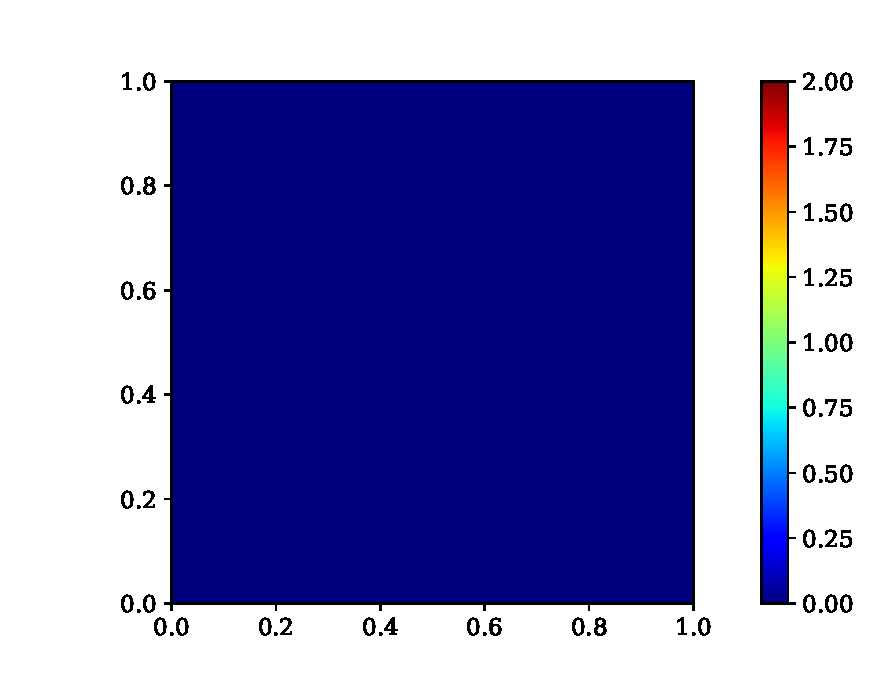
\includegraphics[width=0.5\linewidth]{2sec.pdf}
  \caption{The steady state temperature distribution.}
  \label{fig:sub31}
\label{fig:sub32}
\end{figure}
Since the initial temperature of the plate is $100^{\circ}$C and $\nabla \phi(x,H,t)=0$, the east,west and south boundaries start cooling because of the Dirichlet boundary conditions while part of the north face remains at $100^{\circ}$C. With time, the temperature over the plate starts decreasing in a symmetric way ($x=0.5$ is the axis of symmetry).  As $t \to \infty$, all the points of the plate will be at $0^{\circ}$C.


\end{document}

